\chapter{系统操作}
\section{系统起动}
\begin{itemize}
    \item 在桌面找到\lstinline{multimeter.exe}的快捷方式
    \item 在安装路径根目录找到\lstinline{multimeter.exe}应用程序
\end{itemize}
以上两种方式均可打开本软件。
\section{基本操作}
\subsection{用户登录}
打开本软件后,首先要选择用户模式并登录。本软件有以下两种用户模式:
\begin{itemize}
    \item 普通用户
    \item 高级用户
\end{itemize}
\begin{figure}[htbp]
    \centering
    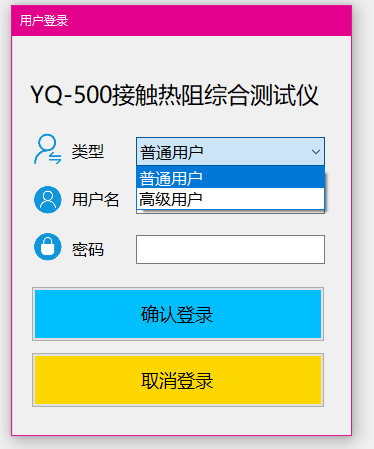
\includegraphics[width=0.6\textwidth]{operation/login.png}
    \caption{ 用户登录 \label{fig:login}}
\end{figure}    
相对\lstinline{普通用户},\lstinline{高级用户}可以进行更多系统级的设置,详见\ref{subsec:advancedUser}一节。
在当前版本中普通用户无需账号密码即可登录,
高级用户的账号密码均为\lstinline{admin}。
在对应栏输入账号密码后,按\lstinline{确认登录}按钮即可进入测试方法选择\ref{subsec:testMethods},
按\lstinline{取消登录}按钮会直接退出本软件。
\subsection{测试方法\label{subsec:testMethods}}
\subsection{切换测试方法}
\subsection{修改参数}
\subsection{运行}
\subsection{温度监控}
\subsection{当前测试}
\subsection{历史测试}
\subsection{导出结果}
\subsection{高级用户模式\label{subsec:advancedUser}}
\subsubsection*{测试修改参数}
\subsubsection*{串口设置修改}
\subsubsection*{标定参数修改}
\section{各种数据}在软件的使用过程中,用户必须与各种数据和信息打交道。为了让用户能
够操作我们的软件,我们必须为用户提供各种结构以及每个数据元素的含义。
有些数据适合在系统操作说明中给出,有些适合在后面的附录中给出,甚至有些除了在
操作说明的同时给出外,还要在附录中给予归纳,这些都由用户手册编写人员根据实际
兄来决定。这些数据包括
输出数据:应当给出软件以何种形式输出的数据的内容和格式,并要求以例样的形式
给予说明。
中间数据〖条件〗:如果我们告诉用户在软件的运行过程中所产生的中间数据的内容
和格式,有助于用户理解软件的使用,则应当给予说明。
数据限制〖条件〗:如果对数据有限制,如数据的大小限制,则应当给予说明。
数据文件〖条件〗:如果要告诉用户我们的软件所使用的某些数据文件的结构有助于
用户理解我们软件的使用,则应给予说明,但应该注意技术保密。如果对数据文件有
所限制,例如每个文件的最大记录数、每个磁盘的最大文件数等,应当给予说明
\section{处理过程}
如果我们简要地给用户描述我们软件对用户的操作、输入的命令
和输入数据的处理过程,有助于用户了解我们软件的使用,则应给予说明
\section{出错处理}
应当给出各种出错情况以及相应的处理措施
\section{操作技术}
有些软件的操作可能需要一定的技术和经验,才能获得满意的结
果,那么应该在用户手册上尽量给出这些技术和经验的描述,或告诉用户如何才能获得
这些技术和经验。例如,在操作SEAS系统作图纸净化处理时,如何选择适当的阀值就是
需要一定的技术和经验的问题。